\chapter{Arrays}
\label{ch:arrays}

\newcommand{\lecnum}{3}
%\newcommand{\lectitle}{Arrays}
\newcommand{\lecturer}{Frank Pfenning, Andr\'e Platzer}

\chapterTAGS{aliasing, array, correctness, loop-invariant, safety}
\maketitle

\begin{preamble}
\noindent
So far we have seen how to process primitive data like integers in
imperative programs. That is useful, but certainly not sufficient to
handle bigger amounts of data.  In many cases we need \emph{aggregate
  data structures} which contain other data.  A common data structure,
in particular in imperative programming languages, is that of an
\emph{array}.  An array can be used to store and process a fixed
number of data elements that all have the same type.

We will also take a first detailed look at the issue of program
\emph{safety}.  A program is \emph{safe} if it will execute without
exceptional conditions which would cause its execution to abort.  So
far, only division and modulus are potentially unsafe operations,
since division or modulus by 0 is defined as a runtime
error.\footnote{Another runtime error is for division or modulus of
  the smallest integer by $-1$.} Trying to access an array element for
which no space has been allocated is a second form of runtime error.
Array accesses are therefore potentially unsafe operations and must be
proved safe.
\end{preamble}

\begin{gram}[Learning Goals]
With respect to our learning goals we will look at the following
notions.
\begin{description}
\item[Computational Thinking:] Developing contracts that establish the
  safety of imperative programs.

  Developing and evaluating proofs of the safety of
  code with contracts.

%\item[Algorithms and Data Structures:]
%
%Fixed-size arrays

\item[Programming:]

  Identifying, describing, and effectively using arrays and
  \lstinline'for'-loops.

\end{description}

% In lecture, we only discussed a smaller example of programming with
% arrays, so some of the material here is a slightly more complex
% illustration of how to use for loops and loop invariants when working
% with arrays.

\end{gram}

\section{Using Arrays}
\label{sec:arrays:using}
\TAGS{array}

When $t$ is a type, then $t$\lstinline'[]' is the type of an array
with elements of type $t$.  Note that $t$ is arbitrary: we can have an
array of integers (\lstinline'int[]'), and an array of booleans
(\lstinline'bool[]') or an array of arrays of characters
(\lstinline'char[][]').  This syntax for the type of arrays is like
Java, but is a minor departure from C, as we will see later in class.

Each array has a fixed size, and it must be explicitly allocated using
the expression \lstinline'alloc_array(t, n)'.  Here $t$ is the type of
the array elements, and $n$ is their number.  With this operation, C0
will reserve a piece of memory with $n$ elements, each having type
$t$.  Let's try in coin:

\begin{lstlisting}[language={[coin]C}]
% coin
C0 interpreter (coin) 0.3.3 'Nickel'
Type `#help' for help or `#quit' to exit.
--> int[] A = alloc_array(int, 10);
A is 0xECE2FFF0 (int[] with 10 elements)
-->
\end{lstlisting}

The result may be surprising: $A$ is an array of integers with 10
elements (obvious), but what does it mean to say $A$ is
\lstinline'0xECE2FFF0' here?  As we discussed in the lecture on
integers, variables can only hold values of a small fixed size, the
\emph{word size} of the machine.  An array of 10 integers would be 10
times this size, so we cannot hold it directly in the variable $A$.
Instead, the variable $A$ holds the \emph{address} in memory where the
actual array elements are stored.  In this case, the address happens
to be \lstinline'0xECE2FFF0' (incidentally presented in hexadecimal
notation), but there is no guarantee that the next time you run
\lstinline'coin' you will get the same address.  Fortunately, this is
okay because you cannot actually ever do anything directly with this
address as a number and never need to either.  Instead you access the
array elements using the syntax \lstinline'A[i]' where $0\leq i < n$,
where $n$ is the length of the array.  That is, \lstinline'A[0]' will
give you element 0 of the array, \lstinline'A[1]' will be element 1,
and so on.  We say that arrays are \emph{zero-based} because elements
are numbered starting at 0.  For example:

\begin{lstlisting}[language={[coin]C}]
--> A[0];
0 (int)
--> A[1];
0 (int)
--> A[2];
0 (int)
--> A[10];
Error: accessing element 10 in 10-element array
Last position: <stdio>:1.1-1.6
--> A[-1];
Error: accessing negative element in 10-element array
Last position: <stdio>:1.1-1.6
-->
\end{lstlisting}

We notice that after allocating the array, all elements appear to be
0.  This is guaranteed by the implementation, which initializes all
array elements to a default value which depends on the type.  The
default value of type \lstinline'int' is 0.  Generally speaking, one
should try to avoid exploiting implicit initialization because for a
reader of the program it may not be clear if the initial values are
important or not.

We also observe that trying to access an array element not in the
specified range of the array will lead to an error.  In this example,
the valid accesses are \lstinline'A[0]', \lstinline'A[1]', $\ldots$,
\lstinline'A[9]' (which comes to 10 elements); everything else is
illegal.  And every other attempt to access the contents of the array
would not make much sense, because the array has been allocated to
hold 10 elements. How could we ever meaningfully ask what its element
number 20 is if it has only 10? Nor would it make sense to ask
\lstinline'A[-4]'. In both cases, \lstinline'coin' and \lstinline'cc0'
will give you an error message telling you that you have accessed the
array outside the bounds.  While an error is guaranteed in C0, in C no
such guarantee is made.  Accessing an array element that has not been
allocated leads to \emph{undefined behavior} and, in principle,
anything could happen.  This is highly problematic because
implementations typically choose to just read from or write to the
memory location where some element \emph{would} be if it had been
allocated.  Since it has not been, some other unpredictable memory
location may be altered, which permits infamous \emph{buffer overflow
  attacks} which may compromise your machines.

How do we change an element of an array?  We can use it on the
left-hand side of an assignment.  We can set \lstinline'A[i] = e;' as
long as $e$ is an expression of the right type for an array element.
For example:


\begin{lstlisting}[language={[coin]C}]
--> A[0] = 5; A[1] = 10; A[2] = 20;
A[0] is 5 (int)
A[1] is 10 (int)
A[2] is 20 (int)
-->
\end{lstlisting}

After these assignments, the contents of memory might be displayed as
follows, where $A = \mathtt{0xECE2FFF0}$:
\begin{center}
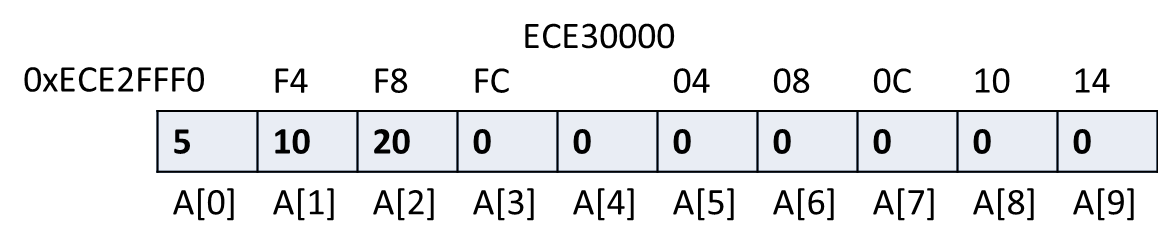
\includegraphics[width=0.85\textwidth]{img/array1.png}
\end{center}

Recall that an assignment (like \lstinline'A[0] = 5;') is a statement
and as such has an effect, but no value.  \lstinline'coin' will print
back the effect of the assignment.  Here we have given three
statements together, so all three effects are shown.  Again, exceeding
the array bounds will result in an error message and the program
aborts, because it does not make sense to store data in an array at a
position that is outside the size of that array.

\begin{lstlisting}[language={[coin]C}]
--> A[10] = 100;
Error: accessing element 10 in 10-element array
Last position: <stdio>:1.1-1.6
-->
\end{lstlisting}


\section{Using For-Loops to Traverse Arrays}
\label{sec:arrays:fors}
\TAGS{array}

A common pattern of access and traversal of arrays is for-loops, where
an index $i$ is counted up from 0 to the length of the array.  To
continue the example above, we can assign $i^3$ to the $i$-th element
of the array as follows:

\begin{lstlisting}[language={[coin]C}]
--> for (int i = 0; i < 10; i++)
... A[i] = i * i * i;
--> A[6];
216 (int)
-->
\end{lstlisting}

Characteristically, the exit condition of the loop tests for
\lstinline'i < n' where $i$ is the array index and $n$ is the length
of the array (here $10$).

After we type in the first line (the header of the for-loop),
\lstinline'coin' responds with the prompt
\lstinline[language={[coin]C}]'...' instead of
\lstinline[language={[coin]C}]'-->'.  This indicates that the
expression or statement it has parsed so far is incomplete.  We
complete it by supplying the body of the loop, the assignment
\lstinline'A[i] = i * i * i;'.  Note that no assignment effect is
printed.  This is because the assignment is part of a loop.  In
general, \lstinline'coin' will only print effects of top-level
statements such as assignments, because when a complicated program is
executed, a huge number of effects could be taking place.


\section{Specifications for Arrays}
\label{sec:arrays:spec}
\TAGS{array, safety}

When we use loops to traverse arrays, we need to make sure that all
the array accesses are in bounds.  In many cases this is evident, but
it can be tricky in particular if we have two-dimensional data (for
example, images).  As an aid to this reasoning, we state an explicit
loop invariant which expresses what will be true on every iteration of
the loop.

To illustrate arrays, we will expand on our previous example, filling
an array with cubes.
%\lstinputlisting{\code/cubes.c0}
\begin{lstlisting}[language={[C0]C}, numbers=left]
int[] cubes(int n) {
  int[] A = alloc_array(int, n);

  for (int i = 0; i < n; i++) {
    A[i] = i * i * i;
  }

  return A;
}
\end{lstlisting}

\noindent
This looks straightforward. Is there a problem with the code or will
it run correctly?  In order to understand whether this function works
correctly, we systematically develop a specification for it.

The first problem is the safety of the call to
\lstinline'alloc_array', because allocating an array will fail if we
ask for a negative number of elements. Since the number of elements we
ask for in \lstinline'alloc_array(int, n)' is $n$, and $n$ is a
parameter passed to the function, we need to add $n \geq 0$ into the
precondition of the function.

For referring to the length of an array, C0 contracts have a special
function \length{(A)} that stands for the number of elements in the
array \lstinline'A'.  Just like the \result{} variable, the function
\length{} is part of the contract language and cannot be used in C0
program code. Its purpose is to be used in contracts to specify the
requirements and behavior of a program.  For the cubes function, we
want to specify the post-condition that the length of the array that
the function returns is $n$.

%\lstinputlisting{\code/cubes2.c0}
\begin{lstlisting}[language={[C0]C}, numbers=left]
int[] cubes(int n)
//@requires n >= 0;
//@ensures \length(\result) == n;
{
  int[] A = alloc_array(int, n);

  for (int i = 0; i < n; i++) {
    A[i] = i * i * i;
  }

  return A;
}
\end{lstlisting}


\section{Loop Invariants for Arrays}
\label{sec:arrays:invariants}
\TAGS{array, loop-invariant, safety}

By writing specifications, we should convince ourselves that all array
accesses will be within the bounds.  In the loop, we access
\lstinline'A[i]', which would raise an error if \lstinline'i' were
negative or greater than \length{(A)}, because that would violate the
bounds of the array.

Because \lstinline'n' is not modified by the loop, we can use our
knowledge that \length{(A) == n} from \lstinline'A''s declaration in
conjunction with the loop guard \lstinline'i < n' to conclude that
\lstinline'i' does not violate the upper bound (i.e., that
\lstinline'i < \length(A)' in each iteration of the loop). For the
lower bound, we need to specify a loop invariant that ensures $i \geq
0$.
\begin{lstlisting}[language={[C0]C}, numbers=left,firstnumber=7]
  for (int i = 0; i < n; i++)
  //@loop_invariant 0 <= i;
  {
    A[i] = i * i * i;
  }
\end{lstlisting}
Operationally, of course, we can reason that because \lstinline'i'
starts at 0 and only increments on every iteration, \lstinline'i'
can't ever be negative.  But in this course we eschew such operational
reasoning, instead encoding this information in loop invariant. We
know that the loop invariant is true initially by the for loop's
declaration: \lstinline'i' is initially 0, and $0 \leq 0$. We
furthermore know that, in an arbitrary iteration of the loop that
initially $i < n$ by the loop guard, so $i' = i+1$ cannot overflow to
a negative number and the loop invariant is always preserved.


\section{Aliasing}
\label{sec:arrays:aliasing}
\TAGS{aliasing, array}

We have seen assignments to array elements, such as %
\lstinline'A[0] = 0;'.  But we have also seen assignments to array
variables themselves, such as

\begin{lstlisting}[language={[C0]C}]
int[] A = alloc_array(int, n);
\end{lstlisting}

What do they mean?  To explore this, we separate the declaration of
array variables (here: $F$ and $G$) from assignments to them.

\begin{lstlisting}[language={[coin]C}]
% coin -d cubes.c0
C0 interpreter (coin) 0.3.3 'Nickel'
Type `#help' for help or `#quit' to exit.
--> int[] F;
--> int[] G;
--> F = cubes(15);
F is 0xF6969A80 (int[] with 15 elements)
--> G[2];
Error: uninitialized value used
Last position: <stdio>:1.1-1.5
--> G = F;
G is 0xF6969A80 (int[] with 15 elements)
--> G = cubes(10);
G is 0xF6969A30 (int[] with 10 elements)
-->
\end{lstlisting}

The first assignment to \lstinline'F' is as expected: it is the
address of an array with 15 elements.  The use of \lstinline'G' in
\lstinline'G[2]', of course, cannot succeed, because we have only
declared \lstinline'G' to have a type of integer arrays, but did not
assign any array to \lstinline'G'.

Afterward, however, when we assign \lstinline'G = F', then
\lstinline'G' and \lstinline'F' (as locals) \emph{hold the same
  address}!  Holding the same address means that \lstinline'F' and
\lstinline'G' are \emph{aliased}.  When we make the second assignment
to \lstinline'G' (changing its value) we get a new array, which is in
fact smaller and definitely no longer aliased to \lstinline'F' (note
the different address).  Aliasing (or the lack thereof) is crucial,
because modifying one of two aliased arrays will also change the
other.  For example:

\begin{lstlisting}[language={[coin]C}]
% coin
C0 interpreter (coin) 0.3.3 'Nickel'
Type `#help' for help or `#quit' to exit.
--> int[] A = alloc_array(int, 5);
A is 0xE8176FF0 (int[] with 5 elements)
--> int[] B = A;
B is 0xE8176FF0 (int[] with 5 elements)
--> A[0] = 42;
A[0] is 42 (int)
--> B[0];
42 (int)
-->
\end{lstlisting}

C0 has no built-in way to copy from one array to another (ultimately
we will see that there are multiple meaningful ways to copy arrays of
more complicated types).  Here is a simple function to copy arrays of
integers.

%\lstinputlisting{\code/copy.c0}
\begin{lstlisting}[language={[C0]C}, numbers=left]
int[] array_copy(int[] A, int n)
//@requires 0 <= n && n <= \length(A);
//@ensures \length(\result) == n;
{
  int[] B = alloc_array(int, n);

  for (int i = 0; i < n; i++)
  //@loop_invariant 0 <= i;
  {
    B[i] = A[i];
  }

  return B;
}\end{lstlisting}

\noindent
For example, we can create $B$ as a copy of $A$, and now assigning to
the copy of $B$ will not affect $A$.  We will invoke coin with the
\lstinline'-d' flag to make sure that if a pre- or post-condition or
loop invariant is violated we get an error message.

\begin{lstlisting}[language={[coin]C}]
% coin copy.c0 -d
C0 interpreter (coin) 0.3.3 'Nickel'
Type `#help' for help or `#quit' to exit.
--> int[] A = alloc_array(int, 10);
A is 0xF3B8DFF0 (int[] with 10 elements)
--> for (int i = 0; i < 10; i++) A[i] = i*i;
--> int[] B = array_copy(A, 10);
B is 0xF3B8DFB0 (int[] with 10 elements)
--> B[9];
81 (int)
--> A[9] = 17;
A[9] is 17 (int)
--> B[9];
81 (int)
-->
\end{lstlisting}


\section{Implementation Note}
\label{sec:arrays:implement}
\TAGS{array, correctness, safety}

Internally, arrays are stored in the area of the memory called the
\emph{heap}.  Memory on the heap is allocated with
\lstinline'alloc_array', which returns the address of an array (and
later in this course \lstinline'alloc' which returns a pointer).  In
C0, memory is not explicitly deallocated, but it is \emph{garbage
  collected} in the sense that memory that can no longer be accessed
from within the running program is freed so that it can be used to
satisfy future allocation requests.

In order to check whether array accesses are in bounds, the C0 runtime
system must store not only the array data, but also the length of the
array.  In the running program, this information cannot be accessed
directly: given an array we cannot obtain its length.  This is mostly
in order to simulate safe programming practices in C.  For example,
when arrays are passed as arguments to functions we usually also pass
(a bound on) their length.

However, in \emph{contracts} (that is, function preconditions
\requires{}, post-conditions \ensures{}, loop invariants
\loopinvariant{} and C0 assertions \assert{}) we can refer to the
length of an array using the special function \length{}.  We have
already used this in the examples above.  For example, the copy
function

\begin{lstlisting}[language={[C0]C}]
int[] array_copy(int[] A, int n)
 //@requires 0 <= n && n <= \length(A);
 //@ensures \length(\result) == n;
 ;
\end{lstlisting}
requires \lstinline'n' to be smaller than the length of the parameter
array \lstinline'A' and ensures that the result array will have length
\lstinline'n'.


\section{Exercises}
\label{sec:arrays:exercises}

\begin{exercise}
  Write a function \lstinline'array_part' that creates a copy of a
  part of a given array, namely the elements from position
  \lstinline'i' to position \lstinline'j'. Your function should have
  prototype
\begin{lstlisting}[language={[C0]C}]
int[] array_part(int[] A, int i, int j);
\end{lstlisting}
Develop a specification and loop invariants for this function.  Prove
that it works correctly by checking the loop invariant and proving
array bounds.
\end{exercise}

\begin{exercise}
  Write a function \lstinline'copy_into' that copies a part of a given
  array \lstinline'source', namely \lstinline'n' elements starting at
  position \lstinline'i', into another given array \lstinline'target',
  starting at position \lstinline'j'. Your function should have
  prototype
\begin{lstlisting}[language={[C0]C}]
int copy_into(int[] source, int i, int n, int[] target, int j);
\end{lstlisting}
As an extra service, make your function return the last position in
the target array that it entered data into.  Develop a specification
and loop invariants for this function.  Prove that it works correctly
by checking the loop invariant and proving array bounds.  What is
difficult about this case?
\end{exercise}

%% I don't believe this is a reasonable question
%% Robert Simmons, December 2014
%% \begin{exercise}
%%   Write a function \lstinline'can_copy_into' that returns an
%%   integer indicating how many elements, starting from position $i$,
%%   of an array $source$ of a given length $n$ can be copied safely
%%   into a part of a given array $target$ starting at position $j$,
%%   into another given array, starting at position $j$. Your function
%%   should have prototype
%% \begin{lstlisting}
%% int can_copy_into(int[] source, int i, int[] target, int j, int n);
%% \end{lstlisting}
%% Develop a specification and loop invariants for this function.
%% Prove that it works correctly by checking the loop invariant and
%% proving array bounds.  The number returned by
%% \lstinline'can_copy_into' should be compatible with the
%% specification of \lstinline'copy_into'.  Which calls to
%% \lstinline'copy_into' are guaranteed to work correctly after a call
%% of
%% \begin{lstlisting}
%% int r = can_copy_into(source, i, target, j, n);
%% \end{lstlisting}
%% \end{exercise}

\begin{exercise}
  Can you develop a reasonable (non-degenerate) and useful function
  with the following prototype? Discuss.
\begin{lstlisting}[language={[C0]C}]
int f(int[] A);
\end{lstlisting}
\end{exercise}
